\section{Organización}

Para enfrentar el actual proceso de acreditación, el Comité Académico del Programa constituyó un
comité ad hoc dedicado a llevar a cabo el presente proceso de autoevaluación. Este comité cuenta
con el apoyo del Departamento de Ingeniería Eléctrica en términos administrativos y financieros.

La Figura 3.1 muestra el organigrama de dicho equipo y está integrado por:

\begin{itemize}
\item Coordinador de Acreditación: Claudio Estévez, Coordinador del Programa, Profesor Asistente.
\item Comité de Acreditación
\begin{itemize}
\item Claudio Estévez, Coordinador del Programa, Profesor Asistente
\item Álvaro Silva, Profesor Colaborador.
\end{itemize}
\item Comité Académico:
\begin{itemize}
\item Claudio Estévez, Coordinador del Programa, Profesor Asistente.
\item César Azurdia, Profesor Asistente
\item Sandra Céspedes, Profesora Asistente
\end{itemize}
\item Equipo Ejecutivo:
\begin{itemize}
\item Jhilmar Molina, Ingeniero Civil Eléctrico.
\item Jorge Flores, Ingeniero Civil Eléctrico.
\item Andrea Canales, Ingeniera Civil Industrial.
\end{itemize}
\item Claustro.
\item Estudiantes del Programa.
\item Egresados del Programa.
\item Institucionalidad:
\begin{itemize}
\item Dirección de Postgrado y Postítulo.
\item Escuela de Postgrado.
\item Otras Direcciones y Escuelas.
\end{itemize}
\end{itemize}

% Figura 3.1

\section{Participación}

Se ha definido el proceso como altamente participativo, en cada etapa se ha considerado la
participación e iteración de los distintos estamentos indicados anteriormente.

\begin{itemize}
\item Se realizó una reunión con las autoridades de la Escuela de Postgrado para dar inicio formal al proceso de autoevaluación.
\item Se realizó una reunión con el Comité Académico para discutir el proceso de acreditación.
\item El comité de acreditación trabajó en forma individual y se reunió en varias ocasiones para discutir el progreso.
\item Se realizaron jornadas informativas donde participó todo el cuerpo académico del Programa.
\item Se informó a los estudiantes activos del Programa que este se estaba acreditando y solicitaba su ayuda y retroalimentación.
\item Se informó a los egresados del Programa que este se estaba acreditando y solicitaba su ayuda y retroalimentación.
\item Se realizaron jornadas de discusión para elaborar el plan de desarrollo con el cuerpo académico del Programa, liderado por el Comité de Acreditación.
\item Se revisa el documento final por todo el cuerpo académico del Programa, recogiendo sugerencias y comentarios.
\end{itemize}


Jornadas participativas:

\begin{itemize}
\item Equipo Acreditación
\item Comité Académico del Programa
\item Claustro
\item Colaboradores
\item Estudiantes del Programa
\end{itemize}

En estas jornadas se presentó la información recabada a lo largo del proceso así como la información consolidada de las encuestas.

\section{Encuestas Acreditación}
\label{encuestas}

El equipo de acreditación en conjunto con la escuela de Postgrado desarrollaron y aplicaron
encuestas a estudiantes, graduados y académicos del Programa. Esto con la finalidad de enriquecer
la autoevaluación e identificar fortalezas y debilidades del Programa. Se presentan a continuación
los resultados más relevantes\footnote{El detalle de las encuestas se encuentra en los anexos y encuestas individuales [\ref{enc_det}]}.

\section{Criterio de Análisis}
\label{criterio_analisis}

Para analizar las encuestas en forma metodológica y objetiva se decide establecer un criterio para
establacer qué aspectos son fortalezas y debilidades. El primer paso es mapear las respuestas a una nota numérica,
como se puede ver en la Tabla \ref{criterio_mapa}. Luego se definen las notas que se consideran fortalezas y debilidades. 
También se ha decidido tener un rango que llamamos ``oportunidad de mejora'', donde el aspecto evaluado 
no se considera como fortaleza o debilidad, sino un punto intermedio. Para efectos del Plan de Desarrollo los aspectos 
que se consideren oportunidades de mejora son como debilidades pero con una prioridad más baja. Las definiciones
de los rangos de las notas se pueden observar en la Tabla \ref{criterio_definicion} y visualmente 
en la Figura \ref{criterios_fig}. Vale la pena mencionar 
que el umbral entre ``De acuerdo'' y ``En desacuerdo'' se encuentra en 2,5. Por este motivo determinamos que los aspectos
que estén en el rango entre 
este umbral (2,5) y la nota mínima (1) se consideran debilidades y del mismo umbral (2,5) hasta la nota 
de ``De acuerdo'' (3) es una oportunidad de mejora. Solo si la nota promedio cae entre ``De acuerdo'' y
``Muy de acuerdo'' se considera una fortaleza. 

\begin{remark} 
Es muy importante destacar que el objetivo del Programa es mejorar en todos los aspectos. Esta medida de categorización es un ejercicio 
para identificar las aspectos que requieren una mejora urgente (debilidades) que se abordarán con alta prioridad y aspectos débiles pero a menor grado (oportunidad de mejora) que se mejorarán con una prioridad secundaria. Incluso, se planea mejorar las fortalezas, pero con una prioridad más baja.
\end{remark}


\begin{table}[!ht]
\centering
\caption{Mapeo de respuesta a notas.}
\label{criterio_mapa}
\begin{tabular}{lc}
\hline
Selección         & Nota \\ \hline \hline
Muy de acuerdo    & 4    \\
De acuerdo        & 3    \\
En desacuerdo     & 2    \\
Muy en desacuerdo & 1    \\
\hline
\end{tabular}
\end{table}

\begin{table}[!ht]
\centering
\caption{Definiciones de fortaleza, debilidad y oportunidad de mejora.}
\label{criterio_definicion}
\begin{tabular}{lc}
\hline
Categoría             & Rango de Notas \\ \hline \hline
Fortaleza             & {[}4 , 3{]}    \\ 
Oportunidad de Mejora & (3 , 2,5{]}    \\ 
Debilidad             & (2,5 , 0{]}    \\ \hline
\end{tabular}
\end{table}

\begin{figure}[!ht]
\centering
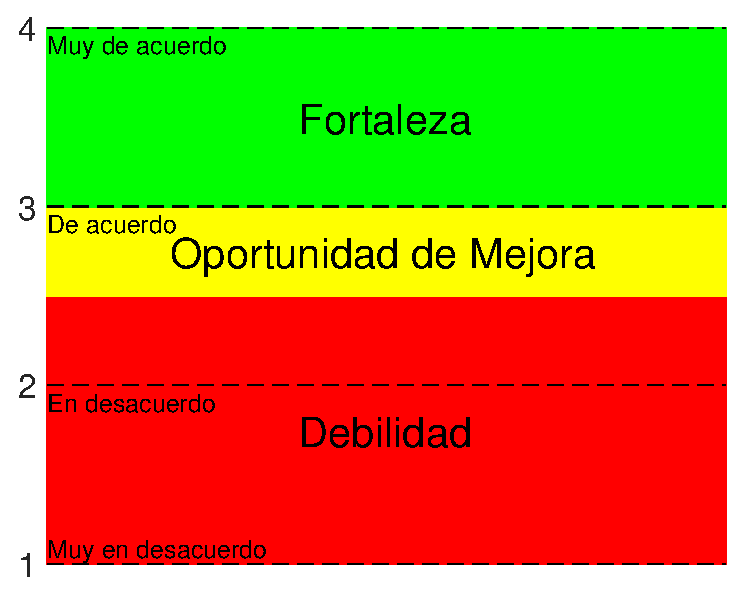
\includegraphics[width=0.5\columnwidth]{./pictures/criterios.eps}
\caption{Definiciones de rango de notas para las categorías de Fortaleza, Debilidad y Oportunidad de Mejora.}
\label{criterios_fig}
\end{figure}




\subsection{Consolidado de las Encuestas}

Primero se presenta un resumen de las estadísticas, de forma que sea fácil de ver donde se 
presentan los problemas más grandes. Utilizando el sistema de notas descrito en la sección previa obtenemos 
los promedios de las distintas categorías por grupo, siendo los grupos: Académicos, Egresados y Estudiantes. 
Estos resultados me muestran en la Figura \ref{encuestas_fig}. Los puntos que corresponden a "Total", 
representan los promedios ponderados (considerando la cantidad de personas que contestaron por grupo) de cada 
categoría. La categoría de Egresados corresponde a preguntas que solo fueron hechas al grupo de los egresados,
por lo que su promedio es el mismo valor y no se graficó. Debajo de la Figura \ref{encuestas_fig} se puede observar
lo que significan los acrónimos del eje horizontal.

Esta vista general muestra que los aspectos que más presentan debilidades son el Apoyo Institucional e Infraestructura (AII) y
la Vinculación con el Medio (VM). Las fortalezas más importantes corresponden a los aspectos de Requisitos de Admisión y 
Proceso de Selección (RAPS), Estructura del Programa y Plan de Estudios (EPPE) y Académicos (Acad). También se puede 
observar que los egresados evaluaron bastante bien el Programa, con casi todos los aspectos entre Muy de acuerdo y De acuerdo.




\begin{figure}[!ht]
\centering
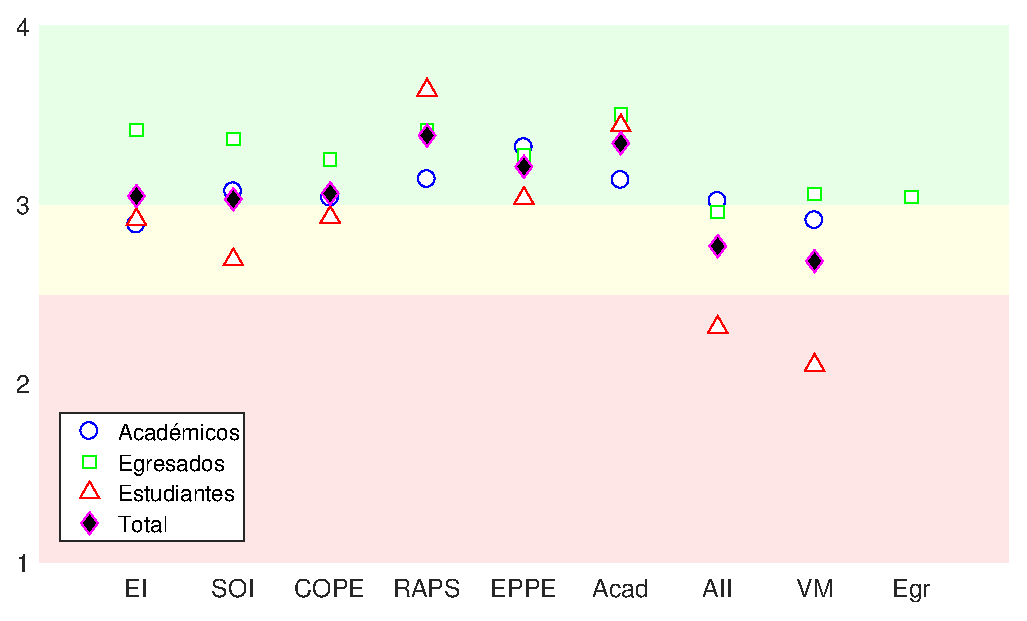
\includegraphics[width=0.8\columnwidth]{./pictures/encuestas.eps}
\caption{Resumen de las encuestas por categoría.}
\label{encuestas_fig}
\end{figure}

\begin{table}[!ht]
\centering
\label{acronyms}
\begin{tabular}{rl}
EI   & Entorno Institucional                         \\
SOI  & Sistema de Organización Interna               \\
COPE & Carácter, Objetivos y Perfil de Egreso        \\
RAPS & Requisitos de Admisión y Proceso de Selección \\
EPPE & Estructura del Programa y Plan de Estudios    \\
Acad & Académicos                                    \\
AII  & Apoyo Institucional e Infraestructura         \\
VM   & Vinculación con el Medio                      \\
Egr  & Egresados                                    
\end{tabular}
\end{table}

\begin{table}[!ht]
\centering
\caption{Información sobre la representatividad de los datos recolectados de las encuestas.}
\label{representatividad_encuestas}
\begin{tabular}{lccc}
\hline
Grupo       & Contestaron & Total & Porcentaje \\ \hline \hline
Académicos  & 8 & 13 & 61,5\% \\
Egresados   & 6 & 8 & 75\% \\
Estudiantes & 7 & 11 & 63,6\% \\
\hline
\end{tabular}
\end{table}


El detalle de cada categoría se presenta en las siguientes secciones. Presentamos los datos en el mismo orden de la encuesta.



\subsubsection{Entorno Institucional}

\noindent\textbf{General}

En el caso del Entorno Institucional (EI), las notas promedio de los 
académicos es de 2,89, de los egresados es de 3,42 
y de los estudiantes es de 2,92, generando el total de 3,05.
Esto indica que esta categoría, en general, es una fortaleza del Programa. Sin embargo, hay aspectos individuales 
que se deben mejorar. 

\noindent\textbf{Individual}

A continuación se enlistan los casos que presentan oportunidades de mejora y debilidades en base a los resultados de la Tabla \ref{entorno_institucional}.

\noindent\textbf{Oportunidades de Mejora:}

\begin{itemize}
\item La normativa que regula el programa de postgrado es clara y conocida
\end{itemize}


\begin{table}[!ht]
\centering
\caption{Resultados encuesta acerca de entorno institucional.}
\label{entorno_institucional}
\begin{tabular}{p{6.2cm}cccc}
\hline
\multicolumn{5}{r}{Promedio de las Encuestas [1-4](4 es mejor o ``Muy de acuerdo'')} \\ \cline{2-5} 
& Académicos  & Egresados & Estudiantes & Total \\
\hline \hline
\begin{tabular}[c]{@{}p{6cm}@{}}La normativa que regula el programa de postgrado es clara y conocida\end{tabular} & 2,63 & 3,33 & 2,83 & 2,9 \\
\hline
\begin{tabular}[c]{@{}p{6cm}@{}}El plan de formación del programa es conocido por los académicos/egresados/estudiantes\end{tabular} & 3,14 & 3,5 & 3 & 3,2 \\ \hline
\end{tabular}
\end{table}


\subsubsection{Sistema de Organización Interna}

\noindent\textbf{General}

En el caso del Sistema de Organización Interna (SOI), las notas promedio de los 
académicos es de 3,07, de los egresados es de 3,37 
y de los estudiantes es de 2,69, generando el total de 3,03.
Esto indica que esta categoría, en general, es una fortaleza del Programa. Sin embargo, hay aspectos individuales 
que se deben mejorar. 

\noindent\textbf{Individual}

A continuación se enlistan los casos que presentan oportunidades de mejora y debilidades en base a los resultados de la Tabla \ref{org_interna}.

\noindent\textbf{Oportunidades de Mejora:}

\begin{itemize}
\item En general, el programa funciona de manera eficiente y ordenada en términos académicos
\item Existen actividades que permiten la coordinación entre los académicos del programa
\end{itemize}

\noindent\textbf{Debilidad:}

\begin{itemize}
\item Se hace un buen seguimiento de los estudiantes
\end{itemize}


\begin{table}[!ht]
\centering
\caption{Resultados encuesta acerca del sistema de organización interna.}
\label{org_interna}
\begin{tabular}{p{6.2cm}cccc}
\hline
\multicolumn{5}{r}{Promedio de las Encuestas [1-4](4 es mejor o ``Muy de acuerdo'')} \\ \cline{2-5} 
& Académicos & Egresados & Estudiantes & Total \\
\hline \hline
\begin{tabular}[c]{@{}p{6cm}@{}}En general, el programa funciona de manera eficiente y ordenada en términos académicos\end{tabular} & 2,86 & 3 & 2,43 & 2,76  \\
\hline
\begin{tabular}[c]{@{}p{6cm}@{}}Cuando tengo un problema siempre recibo la orientación e información adecuada para resolverlo\end{tabular} & 3,43 & 3,33 & 2,57 & 3,11 \\ 
\hline
\begin{tabular}[c]{@{}p{6cm}@{}}Existen actividades que permiten la coordinación entre los académicos del programa\end{tabular} & 2,5 & N/A & N/A  & 2,5 \\
\hline
\begin{tabular}[c]{@{}p{6cm}@{}}En general, la organización administrativa (toma de asignaturas, solicitudes de certificados, etc.) del programa funciona de manera eficiente\end{tabular} & N/A & 3,5 & 2,71 & 3,07  \\
\hline
\begin{tabular}[c]{@{}p{6cm}@{}}Existen instancias de participación de los académicos para la toma de decisiones en temas relevantes del programa (malla curricular, sistemas de evaluación, otros)\end{tabular} & 3 & N/A & N/A & 3 \\ 
\hline
\begin{tabular}[c]{@{}p{6cm}@{}}Los mecanismos para comunicarse con docentes y autoridades eran conocidos por los estudiantes\end{tabular} & N/A & 3,5 & 3,14 & 3,31 \\ 
\hline
\begin{tabular}[c]{@{}p{6cm}@{}}Los canales para comunicarse con los estudiantes son los adecuados\end{tabular} & 3,57 & 3,5 & 3,29  & 3,46 \\
\hline
\begin{tabular}[c]{@{}p{6cm}@{}}Se hace un buen seguimiento de los estudiantes\end{tabular} & N/A & N/A & 2 & 2\\
\hline
\end{tabular}
\end{table}



\subsubsection{Carácter, Objetivos y Perfil de Egreso}
\label{caract_obj_perf_egr}

\noindent\textbf{General}

En el caso del Carácter, Objetivos y Perfil de Egreso (COPE), las notas promedio de los 
académicos es de 3,04, de los egresados es de 3,25 
y de los estudiantes es de 2,93, generando el total de 3,06.
Esto indica que esta categoría, en general, es una fortaleza del Programa. Sin embargo, hay aspectos individuales 
que se deben mejorar. 

\noindent\textbf{Individual}

A continuación se enlistan los casos que presentan oportunidades de mejora y debilidades en base a los resultados de la Tabla \ref{obj_y_perfil}.

\noindent\textbf{Oportunidades de Mejora:}

\begin{itemize}
\item El perfil de graduación del programa es conocido por los académicos
\item El perfil de egreso logra dar cuenta de los objetivos del programa
\end{itemize}


\begin{table}[!ht]
\centering
\caption{Resultados encuesta acerca del Carácter, Objetivos y Perfil de Egreso del Programa.}
\label{obj_y_perfil}
\begin{tabular}{p{6.2cm}cccc}
\hline
\multicolumn{5}{r}{Promedio de las Encuestas [1-4](4 es mejor o ``Muy de acuerdo'')} \\ \cline{2-5} 
& Académicos & Egresados & Estudiantes & Total \\
\hline \hline
\begin{tabular}[c]{@{}p{6cm}@{}}El programa tiene objetivos claros y conocidos\end{tabular} & 3,25 & 3,33 & 2,71 & 3,09  \\
\hline
\begin{tabular}[c]{@{}p{6cm}@{}}Los objetivos son congruentes con el enfoque del programa\end{tabular} & 3,13 & 3,17 & 2,71 & 3 \\ 
\hline
\begin{tabular}[c]{@{}p{6cm}@{}}El perfil de graduación del programa es conocido por los académicos/egresados/estudiantes\end{tabular} & 2,63 & 3,33 & 3 & 2,95  \\
\hline
\begin{tabular}[c]{@{}p{6cm}@{}}El programa tiene un perfil de graduación claro\end{tabular} & 3 & 3,17 & 2,86 & 3 \\ 
\hline
\begin{tabular}[c]{@{}p{6cm}@{}}El perfil de egreso logra dar cuenta de los objetivos del programa\end{tabular} & 3,17 & 2,83 & 2,86  & 2,97 \\
\hline
\begin{tabular}[c]{@{}p{6cm}@{}}Tengo conocimiento acerca de si la orientación del programa es de tipo profesional o académico\end{tabular} & N/A & 3,67 & 3,43  & 3,54 \\
\hline
\end{tabular}
\end{table}



\subsubsection{Requisitos de Admisión y Proceso de Selección}

\noindent\textbf{General}

En el caso del Requisitos de Admisión y Proceso de Selección (RAPS), las notas promedio de los 
académicos es de 3,14, de los egresados es de 3,42 
y de los estudiantes es de 3,64, generando el total de 3,39.
Esto indica que esta categoría, en general, es una fortaleza del Programa. 

\noindent\textbf{Individual}

Ningún aspecto individual presenta debilidades.


\begin{table}[!ht]
\centering
\caption{Resultados encuesta acerca de los requisitos de admisión y proceso de selección.}
\label{admision}
\begin{tabular}{p{6.2cm}cccc}
\hline
\multicolumn{5}{r}{Promedio de las Encuestas [1-4](4 es mejor o ``Muy de acuerdo'')} \\ \cline{2-5} 
& Académicos & Egresados & Estudiantes & Total \\
\hline \hline
\begin{tabular}[c]{@{}p{6cm}@{}}Los alumnos que ingresan al programa son acordes al perfil de egreso y las exigencias  del programa\end{tabular} & 3,14 & 3,5 & 3,57 & 3,39  \\
\hline
\begin{tabular}[c]{@{}p{6cm}@{}}Los requisitos y criterios de admisión al programa son claros\end{tabular} & 3,14 & 3,33 & 3,71 & 3,38 \\ \hline
\end{tabular}
\end{table}


\subsubsection{Estructura del Programa y Plan de Estudios}
\label{estruct_prog_plan_est}

\noindent\textbf{General}

En el caso del Estructura del Programa y Plan de Estudios (EPPE), las notas promedio de los 
académicos es de 3,32, de los egresados es de 3,27 
y de los estudiantes es de 3,03, generando el total de 3,21.
Esto indica que esta categoría, en general, es una fortaleza del Programa. Sin embargo, hay aspectos individuales 
que se deben mejorar. 

\noindent\textbf{Individual}

A continuación se enlistan los casos que presentan oportunidades de mejora y debilidades en base a los resultados de la Tabla \ref{estruct_plan_estudios}.

\noindent\textbf{Oportunidades de Mejora:}

\begin{itemize}
\item Los contenidos entregados en los distintos cursos se encuentran actualizados
\item Las metodologías de enseñanza utilizadas por los profesores permiten alcanzar los objetivos propuestos en cada curso
\end{itemize}


\begin{table}[!ht]
\centering
\caption{Resultados encuesta acerca del estructura del Programa y plan de estudios.}
\label{estruct_plan_estudios}
\begin{tabular}{p{6.2cm}cccc}
\hline
\multicolumn{5}{r}{Promedio de las Encuestas [1-4](4 es mejor o ``Muy de acuerdo'')} \\ \cline{2-5} 
& Académicos & Egresados & Estudiantes & Total \\
\hline \hline
\begin{tabular}[c]{@{}p{6cm}@{}}La periodicidad de las clases y el horario son adecuados para el cumplimiento de los objetivos del programa\end{tabular} & 3,38 & 3,67 & 3,14 & 3,38  \\
\hline
\begin{tabular}[c]{@{}p{6cm}@{}}Los cursos y sus contenidos son pertinentes a las demandas actuales de la disciplina del programa\end{tabular} & 3,38 & 3,17 & 2,86 & 3,15  \\ 
\hline
\begin{tabular}[c]{@{}p{6cm}@{}}Los contenidos entregados en los distintos cursos se encuentran actualizados\end{tabular} & 3,17 & 3 & 2,71 & 2,97   \\
\hline
\begin{tabular}[c]{@{}p{6cm}@{}}Las metodologías de enseñanza utilizadas por los profesores permiten alcanzar los objetivos propuestos en cada curso\end{tabular} & 3,17 & 2,83 & 2,86 & 2,97   \\
\hline
\begin{tabular}[c]{@{}p{6cm}@{}}La forma de evaluación a los estudiantes está basada en criterios establecidos y difundidos al inicio de cada curso\end{tabular} & 3,71 & 3,5 & 3,43 & 3,56  \\ 
\hline
\begin{tabular}[c]{@{}p{6cm}@{}}La forma de evaluación en los cursos promueven el aprendizaje de los contenidos\end{tabular} & 3,14 & 3,17 & 3 & 3,1   \\
\hline
\begin{tabular}[c]{@{}p{6cm}@{}}En los cursos se desarrollan actividades teóricas y prácticas\end{tabular} & 3,57 & 2,83 & 3 & 3,17  \\ 
\hline
\begin{tabular}[c]{@{}p{6cm}@{}}Los procesos de elaboración de tesis están reglamentadas y son conocidos de antemano\end{tabular} & 3,13 & 3,5 & 3,17 & 3,25   \\
\hline
\begin{tabular}[c]{@{}p{6cm}@{}}Las normas de graduación son conocidas y están claramente definidas\end{tabular} & 3,25 & 3,33 & 3,17 & 3,25  \\ 
\hline
\begin{tabular}[c]{@{}p{6cm}@{}}La actividad final de graduación responde adecuadamente al enfoque y perfil de graduación del programa\end{tabular} & 3,29 & 3,5 & 3 & 3,25   \\
\hline
\begin{tabular}[c]{@{}p{6cm}@{}}La relación entre el tiempo real de duración y el tiempo oficial fue correcta\end{tabular} & N/A & 3,5 & N/A  & 3,5  \\
\hline
\end{tabular}
\end{table}



\subsubsection{Académicos}
\label{academicos}

\noindent\textbf{General}

En el caso de criterio relacionado a los académicos (Acad), las notas promedio de los 
académicos es de 3,14, de los egresados es de 3,5 
y de los estudiantes es de 3,44, generando el total de 3,34.
Esto indica que esta categoría, en general, es una fortaleza del Programa. Sin embargo, hay aspectos individuales 
que se deben mejorar. 

\noindent\textbf{Individual}

A continuación se enlistan los casos que presentan oportunidades de mejora y debilidades en base a los resultados de la Tabla \ref{result_acads}.

\noindent\textbf{Oportunidades de Mejora:}

\begin{itemize}
\item El programa realiza mecanismos periódicos de evaluación sobre el desempeño docente de los académicos
\end{itemize}


\begin{table}[!ht]
\centering
\caption{Resultados encuesta acerca de los Académicos del Programa.}
\label{result_acads}
\begin{tabular}{p{6.2cm}cccc}
\hline
\multicolumn{5}{r}{Promedio de las Encuestas [1-4](4 es mejor o ``Muy de acuerdo'')} \\ \cline{2-5} 
& Académicos & Egresados & Estudiantes & Total \\
\hline \hline
\begin{tabular}[c]{@{}p{6cm}@{}}El cuerpo académico de este programa se caracteriza por su conocimiento, información actualizada y manejo teórico respecto a las materias impartidas\end{tabular} & 3,75 & 3,17 & 3,43 & 3,48   \\
\hline
\begin{tabular}[c]{@{}p{6cm}@{}}Los académicos del programa poseen una importante trayectoria académica (publicaciones, investigaciones, docencia)\end{tabular} & 3,29 & 3,67 & 3,43 & 3,45  \\ 
\hline
\begin{tabular}[c]{@{}p{6cm}@{}}El programa realiza mecanismos periódicos de evaluación sobre el desempeño docente de los académicos\end{tabular} & 2,5 & N/A & 3,33 & 2,89   \\
\hline
\begin{tabular}[c]{@{}p{6cm}@{}}El programa tiene una adecuada normativa sobre la incorporación de académicos al programa\end{tabular} & 3 & N/A & N/A & 3  \\
\hline
\begin{tabular}[c]{@{}p{6cm}@{}}El número de académicos era suficiente para la cantidad de estudiantes\end{tabular} & N/A & 3,67 & 3,57 & 3,62   \\
\hline
\end{tabular}
\end{table}



\subsubsection{Apoyo Institucional e Infraestructura}
\label{apoyo_inst_infra}

\noindent\textbf{General}

En el caso del Apoyo Institucional e Infraestructura (AII), las notas promedio de los 
académicos es de 3,02, de los egresados es de 2,96 
y de los estudiantes es de 2,31, generando el total de 2,77.
Esto indica que esta categoría, en general, es una oportunidad de mejora del Programa. Hay varios aspectos individuales 
que deben mejorar. 

\noindent\textbf{Individual}

A continuación se enlistan los casos que presentan oportunidades de mejora y debilidades en base a los resultados de la Tabla \ref{apoyo_infra}.

\noindent\textbf{Debilidad:}

\begin{itemize}
\item Las salas de clases tienen una infraestructura adecuada para el cumplimiento de  los requerimientos académicos y para la cantidad de estudiantes
\item Los laboratorios y/o talleres están correctamente implementados
\item El programa cuenta con mecanismos de apoyos a pasantías, congresos u otras actividades
\item Los convenios de doble titulación con que contaba el programa eran conocidos
\end{itemize}



\begin{table}[!ht]
\centering
\caption{Resultados encuesta acerca del apoyo institucional e infraestructura.}
\label{apoyo_infra}
\begin{tabular}{p{6.2cm}cccc}
\hline
\multicolumn{5}{r}{Promedio de las Encuestas [1-4](4 es mejor o ``Muy de acuerdo'')} \\ \cline{2-5} 
& Académicos & Egresados & Estudiantes & Total \\
\hline \hline
\begin{tabular}[c]{@{}p{6cm}@{}}La Facultad tenía a disposición de los estudiantes espacios para el estudio o realización de trabajos\end{tabular} & N/A & 3,33 & 3  & 3,15  \\
\hline
\begin{tabular}[c]{@{}p{6cm}@{}}Las salas de clases tienen una infraestructura adecuada para el cumplimiento de  los requerimientos académicos y para la cantidad de estudiantes\end{tabular} & 3 & 2,5 & 1,57  & 2,38   \\
\hline
\begin{tabular}[c]{@{}p{6cm}@{}}Los laboratorios y/o talleres están correctamente implementados\end{tabular} & 3 & 2,67 & 1,57  & 2,43  \\ 
\hline
\begin{tabular}[c]{@{}p{6cm}@{}}La Biblioteca permitía un fácil acceso a los recursos bibliográficos (horarios, tiempo de préstamo, rapidez de la atención, disponibilidad de los libros, espacio de lectura, etc.)\end{tabular} & N/A & 3,67 & 3,33   & 3,49  \\
\hline
\begin{tabular}[c]{@{}p{6cm}@{}}La Biblioteca de la Facultad dispone de bibliografía adecuada para los cursos y el trabajo de tesis de los estudiantes, a través de suscripciones a revistas y publicaciones científicas en línea, relevantes para la disciplina.\end{tabular} & 3,5 & 3,33 & 3,17   & 3,34  \\
\hline
\begin{tabular}[c]{@{}p{6cm}@{}}El programa cuenta con mecanismos de apoyos a pasantías, congresos u otras actividades\end{tabular} & 2,57 & 2,25 & 1,8  & 2,22   \\
\hline
\begin{tabular}[c]{@{}p{6cm}@{}}Los convenios de doble titulación con que contaba el programa eran conocidos\end{tabular} & N/A & 3 & 1,75   & 2,33  \\
\hline
\end{tabular}
\end{table}




\subsubsection{Vinculación con el Medio}

\noindent\textbf{General}

En el caso del Vinculación con el Medio (VM), las notas promedio de los 
académicos es de 2,91, de los egresados es de 3,06 
y de los estudiantes es de 2,1, generando el total de 2,68.
Esto indica que esta categoría, en general, es una oportunidad de mejora del Programa. Todos los aspectos individuales 
se deben mejorar. 

\noindent\textbf{Individual}

A continuación se enlistan los casos que presentan oportunidades de mejora y debilidades en base a los resultados de la Tabla \ref{vinc_pais}.

\noindent\textbf{Oportunidades de Mejora:}

\begin{itemize}
\item El programa está vinculado con el medio laboral
\end{itemize}

\noindent\textbf{Debilidad:}

\begin{itemize}
\item El programa tiene visibilidad en el país
\end{itemize}


\begin{table}[!ht]
\centering
\caption{Resultados encuesta acerca de la vinculación con el medio.}
\label{vinc_pais}
\begin{tabular}{p{6.2cm}cccc}
\hline
\multicolumn{5}{r}{Promedio de las Encuestas [1-4](4 es mejor o ``Muy de acuerdo'')} \\ \cline{2-5} 
& Académicos & Egresados & Estudiantes & Total \\
\hline \hline
\begin{tabular}[c]{@{}p{6cm}@{}}El programa tiene visibilidad en el país\end{tabular} & 2,57 & 3 & 1,8  & 2,44  \\
\hline
\begin{tabular}[c]{@{}p{6cm}@{}}El programa está vinculado con el medio laboral\end{tabular} & 3,25 & 3,17 & 2,4  & 2,94  \\ 
\hline
\end{tabular}
\end{table}


\subsubsection{Egresados}

\noindent\textbf{General}

En el caso de criterio relacionado a los egresados (Egr), las notas promedio 
son 3,04.
Esto indica que esta categoría, en general, es una fortaleza del Programa. Sin embargo, hay aspectos individuales 
que se deben mejorar. 

\noindent\textbf{Individual}

A continuación se enlistan los casos que presentan oportunidades de mejora y debilidades en base a los resultados de la Tabla \ref{encuesta_egresados}.

\noindent\textbf{Oportunidades de Mejora:}

\begin{itemize}
\item El programa me permitió acceder a un mejor puesto laboral
\item El programa me permitió mejorar mi renta
\end{itemize}




\begin{table}[!ht]
\centering
\caption{Resultados encuesta de preguntas relacionadas a los egresados.}
\label{encuesta_egresados}
\begin{tabular}{p{10.2cm}c}
\hline
\multicolumn{2}{r}{Promedio de las Encuestas [1-4](4 es mejor o ``Muy de acuerdo'')} \\ \cline{2-2} 
&  Egresados  \\
\hline \hline
\begin{tabular}[c]{@{}p{10cm}@{}}El programa ha mantenido contacto con los egresados\end{tabular} & 3  \\
\hline
\begin{tabular}[c]{@{}p{10cm}@{}}El programa solicita la retroalimentación de los graduados\end{tabular} & 3,4  \\ 
\hline
\begin{tabular}[c]{@{}p{10cm}@{}}El programa me permitió acceder a un mejor puesto laboral\end{tabular} & 2,8  \\ 
\hline
\begin{tabular}[c]{@{}p{10cm}@{}}El programa me permitió mejorar mi renta\end{tabular} & 2,8  \\ 
\hline
\begin{tabular}[c]{@{}p{10cm}@{}}El programa me permitió desempeñarme mejor\end{tabular} & 3,2  \\ 
\hline
\end{tabular}
\end{table}


\subsubsection{Evaluación General}

En esta sección se presenta la oportunidad de estudiar las fortalezas y debilidades del Programa desde una perspectiva más
general. Si somos consistentes con nuestra métrica original, una fortaleza correspondería a una puntuación de 3/4 (75\%). 
Observando la Tabla \ref{result_gen} detectamos dos oportunidades de mejora en aspectos de calidad y satisfacción con la 
formación recibida donde fueron evaluadas con 71,4\% y 69,4\%, respectivamente. Nuestro compromiso es mejorar todas las debilidades y oportunidades de mejora para que los estudiantes activos 
estén satisfechos con la formación recibida y consideren que el Programa es uno de alta calidad. Vale la pena mencionar, que a pesar de 
estas observaciones, los estudiantes recomiendan el Programa.

\begin{table}[!ht]
\centering
\caption{Resultados encuesta acerca de evaluación general del Programa.}
\label{result_gen}
\begin{tabular}{p{6.2cm}ccc}
\hline
% \multicolumn{4}{r}{<@title_graph@>} \\ \cline{2-4} 
& \begin{tabular}[c]{@{}c@{}}Académicos\\(max. 7)\end{tabular} & \begin{tabular}[c]{@{}c@{}}Egresados\\(max. 4)\end{tabular} & \begin{tabular}[c]{@{}c@{}}Estudiantes\\(max. 7)\end{tabular}  \\
\hline \hline
\begin{tabular}[c]{@{}p{6cm}@{}}Los egresados de este programa cuentan con los conocimientos adecuados para las exigencias del entorno laboral\end{tabular} & 6,13/7 (87,5\%) & N/A & N/A   \\
\hline
\begin{tabular}[c]{@{}p{6cm}@{}}A partir de su experiencia, ¿Cuál es su evaluación de la calidad del Programa?\end{tabular} & N/A & 3/4 (75\%) & 5/7 (71,4\%)    \\ 
\hline
\begin{tabular}[c]{@{}p{6cm}@{}}A partir de su experiencia, ¿Cuál es su grado de satisfacción con la formación recibida en Programa?\end{tabular} & N/A & 3.17/4 (79,2\%) & 4.86/7 (69,4\%)    \\ 
\hline
\begin{tabular}[c]{@{}p{6cm}@{}}Recomendaría este programa de postgrado a colegas y/o conocidos\end{tabular} & N/A & 5/6 (83,3\%) Sí & 6.5/7 (92,9\%) Sí   \\ 
\hline
\end{tabular}
\end{table}


Desde un punto de vista más macroscópico podríamos decir que las evaluaciones de la Tabla \ref{result_gen} muestran que todos 
los puntajes son mayores al 70\% demostrando que todos los grupos valoran el esfuerzo del Programa, a pesar de las debilidades u otras 
observaciones que presenta. También nos enorgullece observar los altos porcentajes de estudiantes y egresados que recomienda el Programa. 
El conocimiento de esto en sí es una grata recompensa. Esto es evidencia del gran esfuerzo realizado por todo el cuerpo académico.  

Como resumen se puede apreciar altas evaluaciones así como un alto grado de satisfacción con el Programa. Más
allá de las oportunidades de mejora detectadas tanto en el análisis consolidado de las encuestas como en el proceso de
autoevaluación, tanto a nivel de Programa como a nivel institucional perseguimos la mejora continua como parte de
nuestro sello como Universidad de Chile.


\section{Fortalezas, Debilidades y Oportunidades de Mejora por Criterio}

Es importante mencionar que el Programa está comprometido a mejorar todos los aspectos, no tan solo los que presentan debilidades.
Este sistema de categorización es primordialmente un ejercicio de priorización, o sea, nos indica qué aspectos mejorar primero y 
con más urgencia. Por lo tanto, cuando decimos que una categoría no presenta debilidades, no quiere decir que no intentemos 
mejorarlo. Habiendo dicho esto continuamos el ejercicio de categorizar las fortalezas y debilidades.

\subsection{Entorno Institucional}

\noindent\textbf{Fortalezas:}

\begin{itemize}
\item En términos institucionales hay que destacar que la Universidad de Chile tiene un historial de premios nacionales, de formar 
muchas de las personas que han influenciado mucho en el progreso del país y que han ganado premios nobel. La institución es receptora 
de un gran porcentaje proyectos de investigación y desarrollo. La filosofía académica es y siempre ha sido el traspaso de conocimientos
y formar a las nuevas generaciones. Este alto estándar es una de las fortalezas más importantes de nuestra Universidad, Facultad, 
Departamento y Programa.
\item Las estrictas exigencias de la Escuela de Postgrado de la Facultad y el Departamento de Postgrados y Postítulos de la 
Universidad ha sido un propulsor de calidad en el Programa. 
\item La difusión del plan de formación se ha realizado en forma exitosa ya que la mayoría de los académicos, egresados y 
estudiantes declara conocerlo. Esto se debe, en gran parte, a la orientación que se les brinda al inicio del Programa, la página web y 
por la interacción con otros estudiantes en actividades organizadas por el Programa.
\item Se destaca la existencia de un aparato institucional en distintas instancias para
dar seguimiento a los aspectos operativos y al mismo tiempo permitir la ejecución de políticas estratégicas
con miras a garantizar el continuo mejoramiento de los Programas. A nivel institucional, se encuentra la
Vicerrectoría de Asuntos Académicos (VAA) de la Universidad de Chile. A Nivel de la Facultad de Ciencias
Físicas y Matemáticas se encuentra la Escuela de Postgrado que es la responsable formal de la administración
del Programa (desarrollado en extenso en el Capítulo 2). Finalmente a nivel de la unidad académica está
el Comité Académico cuya principal responsabilidad es llevar adelante y ejecutar las responsabilidades del
Programa, según se detalla en el Reglamento General [\ref{reg_mag_doc}].
\end{itemize}

\noindent\textbf{Oportunidades:}

\begin{itemize}
\item En el contexto del marco regulatorio, la reglamentación y los mecanismos de regulación de los Programas de postgrado de la
Universidad de Chile se pueden aclarar y difundir mejor. A pesar de que esta información está disponible en la página web de la
Facultad es necesario facilitar a los académicos, egresados y estudiantes el acceso a esta información cuando la necesiten.
\item Una oportunidad de mejora también se encuentra en la armonización curricular de la carrera de Ingeniería Eléctrica con el Magíster en Ingeniería de Redes de Comunicaciones.
Este es un punto que nos interesa resolver. Los estudiantes de pregrado han manifestado su interés en tomar cursos del Magíster en Ingeniería de Redes de Comunicaciones. Esto 
presenta una oportunidad de motivar al estudiante a especializarse en un tópico de su interés, dentro del área de las telecomunicaciones.
\end{itemize}



\subsection{Sistema de Organización Interna}

\noindent\textbf{Fortalezas:}

\begin{itemize}
\item Una gran fortaleza en este aspecto son los canales de comunicación internos. El Programa tiene listas de distribución de correos, 
tiene la plataforma web de U-cursos donde se usa activamente el foro y envío de mensajes privados. También existe la opción de tener foros 
solo para el cuerpo docente (profesor y ayudantes). Existe la aplicación de Android/iOS de U-Cursos donde los estudiantes pueden recibir
mensajes instantáneos publicados en el foro. Finalmente, los profesores siempre tienen la opción de llamar a la administración del Programa y 
solicitar difundir algún mensaje por correo al grupo solicitado (un curso específico, todo el Programa, estudiantes del Programa, 
profesores del Programa, egresados, etc.)
\item Los mecanismos para comunicarse con el cuerpo académico del Programa son fáciles y conocidos. Este punto está relacionado al punto anterior.
La plataforma de U-Cursos permite comunicación bidireccional (profesor-estudiante y estudiante-profesor), adicionalmente los estudiantes conocen
los correos de los profesores y también conocen la opción de transmitir un mensaje a través de la administración.
\item El Programa de Magíster en Ingeniería de Redes de Comunicaciones es relativamente pequeño. A pesar de que esto en sí no es una fortaleza, permite un trato más personalizado.
Cuando los estudiantes tienen algún problema contactan al coordinador u algún profesor y se hace el mejor esfuerzo por ayudar a resolver el 
problema, duda, preocupación u otro. 
\item La organización administrativa funciona bien y esto se puede atribuir, nuevamente, al tamaño del Programa y el trato personalizado 
que esto permite. Cuando un estudiante requiere de algún documento, el Programa intenta responder en forma expedita.
\item En términos de generar instancias para reunirse y tomar decisiones, el Programa tiene reuniones periodicas tanto con el claustro como 
con el Comité Académico. A pesar de que este punto se registra como una fortaleza, dado el reducido tamaño del Programa existe una 
oportunidad de mejora para aumentar la periodicidad de las reuniones con la planta colaboradora y otras entidades del DIE. Los colaboradores del Programa tienen 
una increible experiencia que se debe aprovechar, por lo que hay que hacer un esfuerzo para acomodar las reuniones en un horario que facilite 
su participación.
\end{itemize}


\noindent\textbf{Oportunidades de Mejora:}

\begin{itemize}
\item La eficiencia y orden del Programa presenta una oportunidad de mejora. El Programa tiene un calendario separado al de la Facultad. A pesar
de que las fechas de inicio se diseñan para que el Programa comience sus labores docentes en sincronía con los demás cursos del Departamento, 
los cursos del Programa son más concentrados (cada día de clases equivale a las horas de una semana de un curso tradicional). Esto causa que 
los cursos terminen en 9 semanas (en lugar de 15, sin contar examenes). Las actas de los cursos se abren al final del semestre regular, por lo que todos los 
semestres es necesario solicitar que se abran en forma temprana y esto tiende a causar problemas. Para agravar el problema, las actas se abren por 
un periodo típicamente de dos semanas y ocurre que los profesores del Programa (luego de esperar hasta 6 semanas) se distraen y no suben las actas 
en el periodo establecido. Este es uno de los problemas más recurrentes y tenemos propuestas de mejora para el plan de desarrollo.
\item Se declara que escasean actividades que permitan la coordinación entre los académicos del Programa. A pesar de que el Programa 
ha organizado actividades para que los profesores interactúen, incluso junto a los estudiantes y egresados, estas han tenido poca 
participación. En estas instancias se ha logrado recoger valiosa retroalimentación de los estudiantes activos y 
se han generado ideas entre los profesores que han asistido. Es necesario aumentar las instancias donde se inviten exclusivamente a los académicos, con un foco
más formal, donde se discutan las debilidades. Además de generar posibles soluciones, estas instancias sirven para consensuar ideas, para así 
poder ejecutar en forma expedita.
\end{itemize}



\noindent\textbf{Debilidades:}

\begin{itemize}
\item Las encuestas demuestran que no se da seguimiento a los estudiantes. Esto es un punto importante en la formación del estudiante
y debilita la ejecución del plan formativo que moldea a los estudiantes al perfil de egreso que exigimos. Este resultado se puede deber a que 
hay una falta de continuidad al detectar falencias de conocimiento luego de las pruebas. Se le deja caer la responsabilidad sobre el 
estudiante ponerse al día con la materia. A los estudiantes que demuestran dominio de conocimiento también se pueden beneficiar de
una revisión de las pruebas, para así fortalecer más todavía la materia aprendida. Existen varias alternativas 
para mejorar, que serán tratadas en el plan de desarrollo.
\end{itemize}



\subsection{Carácter, Objetivos y Perfil de Egreso}

\noindent\textbf{Fortalezas:}

\begin{itemize}
\item Los egresados y estudiantes conocen muy bien que el Programa es de tipo profesional. Se enfatiza mucho este 
punto al explicarles los objetivos y el motivo por el cual el Programa es vespertino. 
\item En cierta forma relacionado al punto anterior, los distintos grupos conocen el objetivo del Programa. Al ser de carácter 
profesional y tener cursos de regulación, economía y gestión de proyecto, son todos reflejos del objetivo del Programa.
\item Además de estar reflejado en la encuesta, la congruencia entre objetivos y enfoque, por enfoque se puede entender el perfil
de egreso, han sido un punto de mucho esfuerzo y tópico de muchas discuciones en el Comité Académico para crear un Programa que 
genere personas idóneas para llevar a cabo proyectos de telecomunicaciones. La excelencia de los egresados por si solo queremos 
que genere una buena impresión en el mundo laboral. 
\item El perfil de egreso es conocido. Nos preocupamos porque este punto sea claro y no haya ambiguedad. De hecho, este es uno 
de los atractivos del Programa. La multidiciplinariedad del perfil de egreso es una potente combinación en la formación de profesionales.
\end{itemize}

\noindent\textbf{Oportunidades de Mejora:}

\begin{itemize}
\item Se presenta una oportunidad de mejora en la difusión del perfil de graduación. Este punto se debe discutir, puede que sea un 
tema semántico, más que de difusión. En cualquier caso, se presenta como una oportunidad de mejora.
\item El punto de si el perfil de egreso logra dar cuenta de los objetivos del Programa es una oportunidad de mejora. Es importante que 
los objetivos estén bien orientados al perfil de egreso. Dado que la pregunta de si el perfil de egreso es conocido obtuvo también una puntaje 
donde existe una oportunidad de mejora, tal vez el problema sea de difusión del perfil más que de si los objetivos están bien orientados. 
\end{itemize}



\subsection{Requisitos de Admisión y Proceso de Selección}

\noindent\textbf{Fortalezas}

\begin{itemize}
\item El proceso de selección apunta a que los postulantes que ingresan estén bien preparados con los requisitos básicos que exige 
el Programa para poder tener un buen desempeño. Nos apoyamos bastante de la calificación escolar internacional para determinar el 
nivel de desempeño de los estudiantes extranjeros y tratar de entender como comparar los distintos sistemas de evaluación de países 
extranjeros. Existen instancias donde hay países donde sus instituciones tienen distintas bases de notas. Es nuestra responsabilidad y 
compromiso deducir las capacidades de los postulantes en base al material solicitado.
\item Todos los requisitos de postulación se encuentran difundidos en la misma plataforma de postulación. Cualquier duda que exista, la plataforma
además provee los contactos de los coordinadores y de la administración de todos los Programas.
\end{itemize}

No se observan debilidades.

\subsection{Estructura del Programa y Plan de Estudios}

\noindent\textbf{Fortalezas:}

\begin{itemize}
\item Es rutinario difundir información básica el primer día de clases, esto incluye la forma de evaluación.
\item El Programa es de naturaleza vespertina, o sea de 6:30 a 9:30pm, y la duración de estos bloques se intenta aprovechar 
lo máximo posible. Los estudiantes tienen clases todos los días en el bloque mencionado  e incluso los sábados en las mañanas.
Este horario tan denso hace que la periodicidad de las clases no pueda ser más frecuente de lo que ya es (sin acortar las horas 
por curso).
\item A partir del 2013, se hicieron cambios al Programa y se ha tratado de mejorar (acortar) las estadías en el Programa. A
pesar de que se registra como una fortaleza, esto se incluira en el plan de desarrollo para intentar reducir más el tiempo de 
las estadías en el Programa. Hoy día no existen herramientas para ejercer presión.
\item El proceso de elaboración de tesis está reglamentado. Esto incluye fechas límites, tiempos de corrección, requisitos, etc. 
Hoy día hasta se exige un formato normalizado.
\item Este punto presentó problemas en el pasado, pero hoy día existe una plataforma web que permite a los estudiantes ver claramente
que cursos les faltan y la cantidad de UD que necesitan para completar los requerimientos. 
\item La actividad final, en este caso la defensa de tesis, es parte del Reglamento del Programa y exigido por la Facultad. Están diseñados 
para suplir al estudiante de muchas fortalezas, no solamente del punto de vista académico, sino también para que aprendan habilidades blandas.
\item Los cursos tienen un buen balance de actividades prácticas y teóricas. En general, los dos aspectos son importantes para la mejor
compresión del material.
\item Las evaluaciones del curso están diseñadas para evaluar las fortalezas y debilidades de los estudiantes. Se motiva a que se realizen
exactamente dos, pero los profesores tienen completa libertad de realizar más o menos pruebas. Dos pruebas permite dividir el material 
y de forma que si a un estudiante le va mal en una prueba, tenga al menos una oportunidad de subir la nota. Por otro lado, se sugiere no dar más de dos, 
debido a que el Programa (por ser vespertino) no tiene un horario auxiliar y realizar pruebas resta tiempo de cátedra.
\item El área de las telecomunicaciones cambia muy rápidamente, cursos LTE 4G, que se diseñaron en los últimos dos años ya se vuelve obsoleto.
Para mantener el curso actualizado es necesario crear cursos (o modificar los cursos) todos los años. En los últimos 5 semestres se han 
creado 4 cursos. Incluso, en el presente, ya falta poco tiempo para que salgan las especificaciones de 5G. Cuando esto suceda hay que 
evaluar hasta cuando se dictará el curso de la tecnología predecesora. Todo esto dificulta mantener el Programa al día con las tecnologías y en paralelo velar por la calidad de los nuevos cursos.
\end{itemize}

\noindent\textbf{Oportunidades de Mejora}

\begin{itemize}
\item Se percibe como una oportunidad de mejora actualizas los contenidos entregados en los distintos cursos. A pesar de esforzarnos por mantener el material educativo de los distintos cursos del Programa actualizados, en general, esta tarea 
no es trivial. La calidad se tiene que priorizar sobre la rapidez. Sin embargo, no siempre es fácil determinar cuando un curso está listo para
su estreno y han habido casos donde se estrenan cursos que no estaban listos. Se mejorará en este aspecta la frecuencia con que se revisa si el material del curso está actualizado.
\item Otro aspecto que pueden mejorar son las metodologías de enseñanza utilizadas por los profesores. Cada profesor tiene sus técnicas de docencia. Hay profesores que solo usan la pizarra, otros que en forma constante solicita a estudiantes
desarrollar algún problema en la pizarra, otros intentan enriquecer con charlas técnicas de empresarios. Hay verificar que la metodología es la apropiada para alcanzar los objetivos del curso. Para esto hay que involucrar a expertos de metodología de enseñanza, los cuales existen en la Facultad, y pueden ayudar junto a los profesores de los cursos a revisar los programas.
\end{itemize}



\subsection{Académicos}

\noindent\textbf{Fortalezas:}

\begin{itemize}
\item El cuerpo académico se caracteriza por sus conocimientos, en particular por la multidiciplinariedad que provee. El cuerpo 
docente es muy diverso y cubre desde las telecomunicaciones, hasta temas de regulación, economía y gestión de proyecto.
\item El cuerpo docente posee una larga historia de trabajar en instituciones privadas o en Canadá. Los años de experiencia por 
profesor es extensa. La mayoría ha trabajado en proyecto de telecomunicaciones. Las consultorias hechas también son un indicador de la experiencia que posee la planta de académicos del Programa.
\item La cantidad de profesores por estudiantes siempre ha sido baja, incluso en ocasiones hay más profesores que estudiantes en el Programa.
\item El Programa, como cualquier otra unidad institucional, debe hacer las contrataciones en forma transparente. La Universdiad tiene una 
estricta política de contratación. El Decano es la persona que finalmente decide que académicos son contratados y cuales no.
\end{itemize}


\noindent\textbf{Oportunidades de Mejora}

\begin{itemize}
\item La evaluación de los académicos es fundamental. Existe una plataforma en línea que se provee para evaluar a los profesores. 
Esto se hace dos veces por semestre. La plataforma permite hacer comentarios.
\end{itemize}



\subsection{Apoyo Institucional e Infraestructura}

\noindent\textbf{Fortalezas:}

\begin{itemize}
\item Dentro de la Facultad existen espacios apropiados para el estudio, incluyendo en la biblioteca. En el Departamento
también existen espacios, incluyendo la misma sala que se usa para dar clases. Esta sala es de uso exclusivo para estudiantes
del Magíster en Ingeniería de Redes de Comunicaciones.
\item La biblioteca cuenta con una extensiva variedad de libros y en los casos que no se encuentra, existe la posibilidad 
de ordenar libros. La biblioteca además tiene las bases de datos digitales necesarias para poder estudiar trabajos de algún área 
en específico. La bibliografía es adecuada para los cursos del Programa y para el desarrollo de la tesis.
\end{itemize}

\noindent\textbf{Debilidades:}

\begin{itemize}
\item Las salas de clase no tienen una infraestructura adecuada para el cumplimiento de los requirimientos académicos y para la cantidad de estiduantes. Un problema recurrente que hemos tenido en el Programa es la falla de los proyectores. Estos dispositivos tienen una vida muy corta
y el extenso uso que se le da en los cursos hace que se agrave la situación. Es necesario estudiar alternativas de tecnologías más estables,
como por ejemplo los televisores. 
\item Los laboratorios y/o talleres no están correctamente implementados. En el Departamento de Ingeniería Eléctrica, en general, existen grandes problemas con la red. Es muy inestable. Para cualquier otro Programa, esto puede que no sea 
un problema importante, pero en el Magíster en Ingeniería de Redes de Comunicaciones la red es muy importante, en algunos casos esencial para poder llevar a cabo la experiencia de ese día. Otros problemas que se detectaron es que Microsoft brindó licencias educacionales (gratuitas), que luego de diseñar un laboratorio las canceló. Todo el material docente preparado se perdió y causaron atrasos inesperados, donde los estudiantes compresiblemente no toleraron.
\item Se detecta que el programa no cuenta con mecanismos de apoyos a pasantías, congresos u otras actividades. El Programa, actualmente, no cuenta con apoyos a conferencias ni a pasantías. Este punto se debe estudiar bien del punto de vista financiero, antes de llevar a cabo una solución.
\item Los convenios de doble titulación con que contaba el programa no eran conocidos. El Programa no cuenta con convenios de doble titulación, por lo que se debe hacer un esfuerzo más grande por difundir esta información. 
\end{itemize}



\subsection{Vinculación con el Medio}

\noindent\textbf{Fortalezas:}

\begin{itemize}
\item Los profesores del Programa tienen un fuerte vínculo con el medio externo. Esto incluye participación internacional en proyectos, 
colaboración en publicaciones, tanto en revistas como en conferencias, participación de eventos nacionales e internacionales, organización de 
conferencias en el área de ingeniería eléctrica, etc. El problema que se detecta es que hay que fomentar más la participación de los 
estudiantes en estas iniciativas. De esta forma, no solo se involcran más los estudiantes con estos vínculos, sino que enriquece más el proceso formativo 
de los estudiantes.
\end{itemize}

\noindent\textbf{Oportunidades de Mejora}

\begin{itemize}
\item El Programa no ha hecho un esfuerzo suficientemente grande para mantener un buen vínculo con las empresas. Se necesitan 
generar más oportunidades de cooperación, como lo son convenios y trabajos dirigidos.                                                     
\end{itemize}

\noindent\textbf{Debilidades:}
\begin{itemize}
\item La encuesta revela que se considera que el Programa no tiene un fuerte vínculo con el país. Como se discute en la 
Sección \ref{vinculacion_medio}, el Programa tiene un fuerte vínculo con otras organizaciones externas, principalmente 
con otras universidades. Por medio de proyectos con participación internacional, colaboraciones con iniciativas académicos, 
organización de conferencias, etc. El claustro tiene una ámplia red de contactos. El cuerpo académicos de colaboradores 
tiene, también, una extensa red de contactos, pero a diferencia del claustro estos vínculos son con la empresa privada e 
instituciones gubernamentales que tratan temas de telecomunicaciones. El problema que detectamos es que es necesario hacer 
la participación de los estudiantes más activa, no tan solo para ayudarlos con los vínculos con el medio, sino que ayuda 
a los estudiantes a desenvolverse mejor ante profesionales del área.
\end{itemize}

\subsection{Egresados}

\noindent\textbf{Fortalezas:}

\begin{itemize}
\item El Programa ha hecho un buen trabajo de mantenerse en contacto con sus ex-alumnos. Muchos estudiantes del Programa son del extranjero 
y cuando visitan a Chile a veces despejan tiempo para venir a ver s sus ex-profesores.
\item Cuando los estudiantes egresan le solicitamos retroalimentación en forma constante, no es obligatorio pero se les informa a 
los egresados que esto es para mejorar el Programa y esa información es muy valiosa.
\item La formación brindada a los alumnos les permite desempeñarse mejor una vez egresan. 
\end{itemize}

\noindent\textbf{Oportunidades de Mejora:}

\begin{itemize}
\item A pesar de que el acceso a mejores puestos laborales depende mucho de factores externos al Programa, se analizará internamente 
como poder mejorar este aspecto.
\item Similar al punto anterior, mejorar la renta de los egresados es un factor externo al Programa, que a pesar de que es dependiente de las 
destrezas aprendidas, no es el único factor. Sin embargo, se analizará como se podría mejorar este aspecto.
\end{itemize}



\section{Plan De Desarrollo}
\label{plan_de_desarrollo}

El Plan de Desarrollo responde al desarrollo estratégico del Programa así como a las fortalezas, debilidades y
oportunidades detectadas a lo largo del proceso de autoevaluación. Para la elaboración de la Tabla \ref{table_plan_desarrollo},
que resumen este plan, se elabora una descripción general del conjunto de medidas centrales que se propone llevar
a cabo en el corto y mediano plazo. Para ello cada medida es identificada con su nombre, una descripción general, su
objetivo y de qué forma se hace cargo de las debilidades y oportunidades evidenciadas. Se destaca en el diseño del Plan
de Desarrollo una visión sistémica, donde más que un conjunto de medidas aisladas que ataquen debilidades puntuales,
se privilegia el desarrollo de medidas macro que apunten a superar un conjunto de debilidades (y potencien fortalezas),
cuando sea posible.

\begin{table}[!ht]
\centering
\caption{Plan de Desarrollo sobre debilidades detectadas}
\label{table_plan_desarrollo}
\begin{tabular}{p{0.2\columnwidth}p{0.2\columnwidth}p{0.2\columnwidth}p{0.2\columnwidth}p{0.2\columnwidth}} 
% p{6.2cm} p{0.5\columnwidth} \begin{tabular}[c]{@{}p{10cm}@{}}   \end{tabular}
\hline 
Debilidad & Acción & Indicadores & Plazos & Responsables \\ \hline \hline 

Seguimiento a los estudiantes  &  Identificar / Repasar  &  Encuestas u-cursos   &  Inmediatamente  &  Todos los profesores   \\ \hline 
Infraestructura en las salas  &  Buscar alternativas   &  Existencias de nuevas quejas  &  Primer semestre 2018 &  Comité Académico  \\ \hline 
Implementación de laboratorios &  Mejorar / Alternativas locales  &  Encuestas u-cursos  &  2018  &  Comité Académico  \\ \hline 
Apoyo a actividades   &  Discusión sobre Inversión  &  Actividades asistidas apoyadas por el Programa   &  Primer Semestre 2018  &  Comité Académico  \\ \hline 
Convenios doble titulación &  Orientaciones Internas &   Encuestas &  Inmediatamente &  Todos los profesores  \\ \hline 
Vínculo con el Medio & Integración & Cantidad de estudiantes involucrados en actividades externas & Inmediatamente & Todos los profesores \\
\hline 
\end{tabular}
\end{table}


\subsection{Ejecución del Plan de Desarrollo que aborda las Debilidades}

\subsubsection{Seguimiento a los Estudiantes}

Se identidica como una debilidad el seguimiento a los estudiantes. En este aspecto los profesores del Programa han acordado aumentar el 
compromiso con los estudiantes. 

Hay dos medidas de acción principales: 

\begin{enumerate}
\item Identificar a los estudiantes que presentan mayor dificiltad de aprendisaje y apoyarlos. 
\item Resolver las pruebas el primer día de clase que siga a la prueba. 
\end{enumerate}

El apoyo del primer punto puede venir de varias formas, aquí se mencionan algunos ejemplos pero no están restringidos a estos.

Medidas de apoyo:
\begin{itemize}
\item Sentarse con el estudiante y revisar aspectos débiles
\item Asignar tareas adicionales y revisarlas con el estudiante
\item Pedirle al estudiante que prepare una presentación explicando el tema que presenta debilidad e identificar fallas
\end{itemize}

En relación al segundo punto, este ayudaría a darle seguimiento a los estudiantes que tienen buen desempeño, además de los que presentan 
debilidades. Esta sería una medida más transversal.


\subsubsection{Infraestructura en las Salas}

Este ítem requiere un análisis de parte del Comité Académico del Programa. Este es un problema relativamente pequeño, pero su solución podría
tener un gran impacto. El Comité Académico debe decidir primero si las clases deben continuar en la sala actual, conocida como la sala de 
postítulo, o si se mueve a las nuevas facilidades de la Facultad en Beauchef 851. Ambas alternativas tienen ventajas y desventajas. De decidir mantener la sala actual, le sigue la discusión de que equipo comprar: proyector, monitor, televisión, etc. Se espera que la decisión esté tomada para marzo y pueda ser ejecutada ese mismo mes.

\subsubsection{Implementación de Laboratorios}

Antes de ejecutar cualquier plan hay que solicitarle a los profesores que tienen laboratorios que le describan al Comité que experiencias han 
exibido problemas y cuales son los factores. Se identifica que la irregularidad de la Internet entorpece el flujo de las experiencias. Dado que se estudien bien los factores principales que causan problemas, se puede invertir en mejoras. Una alternativa que está considerada es instalar un servidor local en la sala de clases. De esta forma, si la Internet presenta problemas, esto no afectaría la experiencia ya que se independizaron de la Internet en este aspecto.

\subsubsection{Apoyo a Actividades}

Se ha decidido crear un fondo de apoyo a actividades externas, particularmente conferencias. Los fondos serán concursables. Las métricas de evaluación se difundirán una vez sean consensuadas. Estas métricas serán diseñadas para fortalecer otros aspectos del Programa, por ejemplo,
no necesariamente la medida que se tomará, el estudiante que gane el concurso de ``viaje a conferencia'' debe comprometerse a formar parte 
de un grupo de tutores que ayuden a darle seguimiento a los estudiantes que presenten dificultades para entender un tópico en particular.

\subsubsection{Convenios de doble títulación}

Este es un problema de difusión y su solución es idéntica a la presentada en la Sección \ref{difusion}.


Esto resume los aspectos más debiles del Programa. Ahora se pasará a discutir las oportunidades de mejora que se identifican en base a las encuestas.



\begin{table}[!ht]
\centering
\caption{Plan de Desarrollo sobre oportunidades de mejora detectadas}
\label{table_oportunidades_mejora}
\begin{tabular}{p{0.2\columnwidth}p{0.2\columnwidth}p{0.2\columnwidth}p{0.2\columnwidth}p{0.2\columnwidth}} 
% p{6.2cm} p{0.5\columnwidth} \begin{tabular}[c]{@{}p{10cm}@{}}   \end{tabular}
\hline 
Oportunidad & Acción & Indicadores & Plazos & Responsables \\ \hline \hline 

Eficiencia y orden  &  Identificar Problemas / Llevar a cabo &  Generar lista / Ejecutar  &  Primer semestre 2018, continuo &  Crear comité  \\ \hline 
Actividades de coordinación  &  Agendar  &   Asistencia de Profesores   &  Semestral  &  Todos los profesores   \\ \hline 
Difusión del Perfil de Egreso  &  Orientaciones Internas &   Encuestas   &  Primer Semestre 2018  &  Todos los profesores \\ \hline 
Perfil de Egresa da cuenta de los objetivos  &  Analizar fallas  &   Encuestas a empleadores    &  Anual  &   Comité Académico   \\ \hline 
Actualizar Contenido 	&    Revisar contenido    &   Solicitar cambios realizados  &  Semestral  &   Todos los profesores   \\ \hline 
Metodologías de Enseñanza &   Identificar fallas   &   Encuestas U-Cursos   &  Semestral  &   Comité Académico / Todos los profesores   \\ \hline 
Mecanismos de Evaluación de Docentes  &  Levantar información sobre debilidades específicas  &   Encuestas U-Cursos   &  Semestral  &   Comité Académico  \\ \hline 
Vínculo con Medio Laboral  & Integración & Cantidad de estudiantes involucrados en actividades externas & Inmediatamente & Todos los profesores \\ \hline 
Mejores puestos laborales  &  Analizar  &   Formulario + Encuesta de salida   &  Semestral  &   Comité Académico   \\ \hline 
Mejorar la renta  &  Analizar  &   Formulario + Encuesta de salida   &  Semestral  &   Comité Académico   \\
\hline 
\end{tabular}
\end{table}

\subsection{Ejecución del Plan de Desarrollo que aborda las Oportunidades de Mejora}

\subsubsection{Eficiencia y Orden}
\label{eficiencia_orden}

Este punto se decide dividir en tres partes de ejecución:

\begin{enumerate}
\item Identificar cuales son los problemas principales de eficiencia
\item Diseñar un plan de mejora de eficiencia
\item Llevar a cabo el plan 
\end{enumerate}

El primer punto se llevará a cabo inmediatamente. El objetivo es empezar a ejecutar el plan de mejora a más tardar el semestre que viene.

Algunos temas ya consensuados por el cuerpo académico son: 

\begin{itemize}
\item Reunir al cuerpo académico completo bianualmente y discutir aspectos débiles, socializar el calendario del Programa. Incluso entre los profesores que no tengan clase ese semestre, de forma que puedan ir actualizando su materia y preparando el material de apoyo.
\item Monitorear las horas en que los profesores llegan a clases, por medio de un registro de asistencia con sello de tiempo.
\item Incentivar a los profesores a obtener puntajes altos en las evaluaciones del curso.
\end{itemize}



\subsubsection{Actividades de Coordinación}

Como se menciona en la sección anterior, el cuerpo académico se reunirá bianualmente para discutir aspectos que se consideran débiles, difundir el calendario, presentar informes de progreso (si aplican), conversar sobre tecnologías emergentes y decidir si queremos incorporar nuevos cursos al Plan de Estudio.


\subsubsection{Difusión del Perfil de Egreso}
\label{difusion}

Este problema es de difusión. Aquí se presenta una interesante oportunidad de mejora. El plan es tener una charla de orientación, separada de la 
orientación que provee la Facultad, donde se expliquen entre otras cosas:

\begin{itemize}
\item El perfil de egreso
\item El plan de estudio
\item Tiempos sugeridos
\item Cuando deben decidir con qué profesor trabajar
\item Dar una breve descripción de los cursos
\item Informar sobre convenios de doble titulación (si no existen mencionar que no existen)
\end{itemize}

La parte interesante es que la charla será dictada por todos los profesores del curso en forma rotativa. Esto logra que no tan solo los estudiantes 
estén informados, sino que fuerza a los profesores a estarlo también.


\subsubsection{Actualizar Contenido}

En el Programa de Magíster en Ingeniería de Redes de Comunicaciones es particularmente importante mantener los cursos actualizados. El Programa es de carácter tecnológico y no 
es aceptable que esté desactualizado. Como se menciona en la Sección \ref{eficiencia_orden}, la instancia para actualizar la materia de los cursos 
es el semestre anterior. Para saber que semestre se dicta un curso en particular, los profesores deben asistir a las reuniones bianuales mencionadas previamente.

\subsubsection{Metodologías de Enseñanza}

La metodología de enseñanza es esencial para un traspaso de información eficiente. Se ha decidido solicitar a una experta en estrategias de metodología docente que revise los Programas de los cursos del Programa y nos sugiera que herramientas 
se pueden usar para mejorar el flujo de información. 

\subsubsection{Mecanismos de Evaluación de Docentes}

Este mecanismo ya existe. La plataforma de U-Cursos provee herramientas para evaluar a los profesores dos veces por semestre. La primera encuesta se hace entre la séptima y octava semana del semestre y la segunda encuesta se hace al final del semestre. Cuando los cursos han registrado problemas se ha intervenido. Esto solo a ocurrido tres veces desde el 2013.

\subsubsection{Vínculo con el Medio Laboral}

El problema identificado no es la carencia de vínculos con el medio externo, ya que todos los profesores 
del Programa tiene una increíble red de colaboradores. El problema es que no se han involucrado a los estudiantes.
Esto se puede resolver fácilmente involucrando más a los estudiantes en los proyectos internacionales, promover la asistencia a actividades 
de telecomunicaciones, como los son los Smart Cities Summits, por ejemplo. Cuando los estudiantes asisten a estas conferencias se vinculan más con
proyectos tecnológicos. Si se incorporan formalmente a un proyecto, están practicando obligados a interactuar con colaboradores internacionales.

\subsubsection{Mejoras de Puestos laborales/Renta}

Las últimas dos oportunidades de mejora están fuertemente relacionados. Este problema tiene un factor externo considerable. Incluso se podría argumentar que la economía de la nación, la oferta de trabajo, el mercado, los proyectos gubernamentales, etc. tienen tanto impacto como la formación
que provee el Programa. 
Sin embargo, en un esfuerzo de mejorar este punto, se informará a los estudiantes de ferias de trabajo y otras oportunidades de entrevistas, donde
puedan participar.


















